\chapter{Introduction}
\label{chap:intro}
\section{Figure Examples}
\subsection{One Figure}
Figure~\ref{fig1} shows Pluto's image captured by New Horizons. 
\begin{figure*}[htb!]
\center
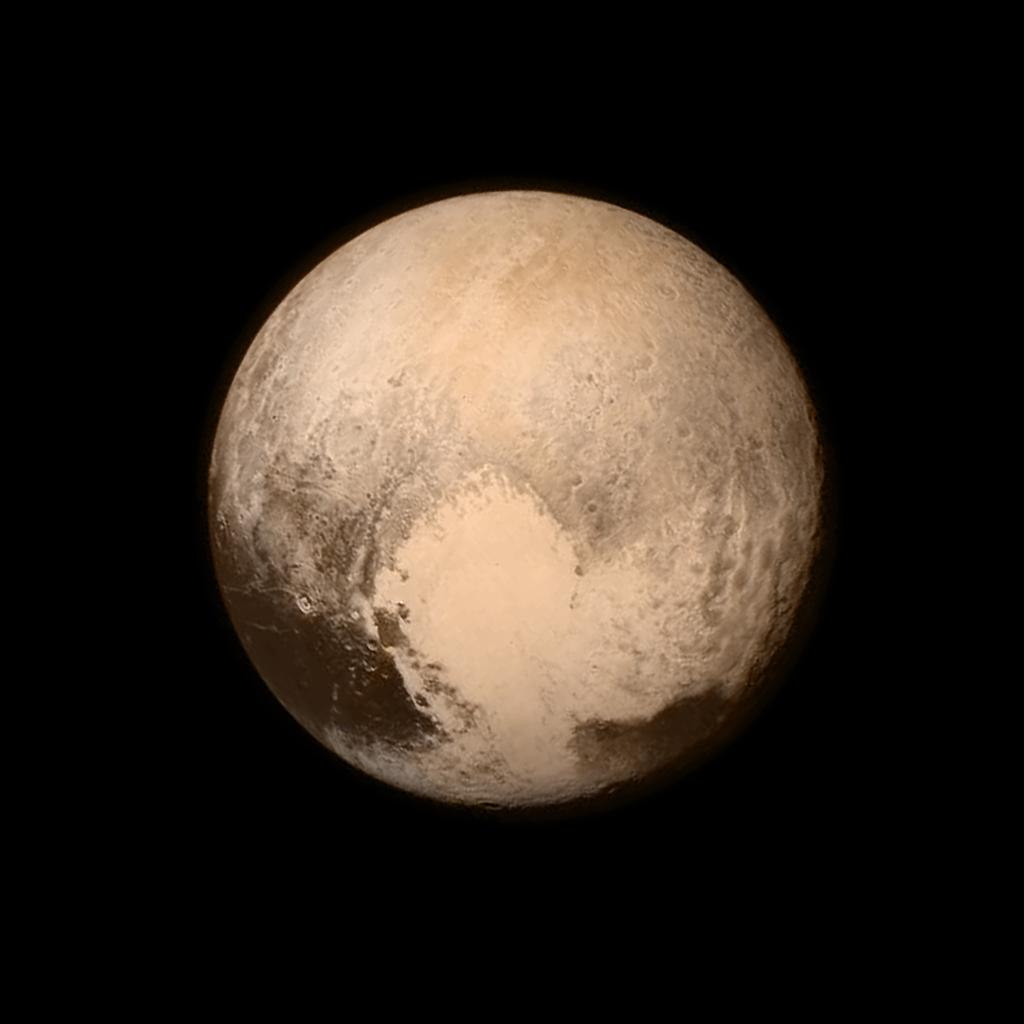
\includegraphics[width=0.5\textwidth]{figures/PIA19708-orig.jpg}
\caption[Shot description of the figure 1.1.]{Long description of figure 1 (Pluto captured by New Horizons). Note: there is a short description which will show on your list of figures. Image taken from \url{https://images-assets.nasa.gov/image/PIA19708/PIA19708~orig.jpg}.}
\label{fig1}
\end{figure*}

\subsection{One Horizontal Figure}
Figure~\ref{fig2} is an example of landscape image, which is Ultima Thule captured by New Horizons extended mission.


\begin{landscape}
\begin{figure*}[htb!]
\center
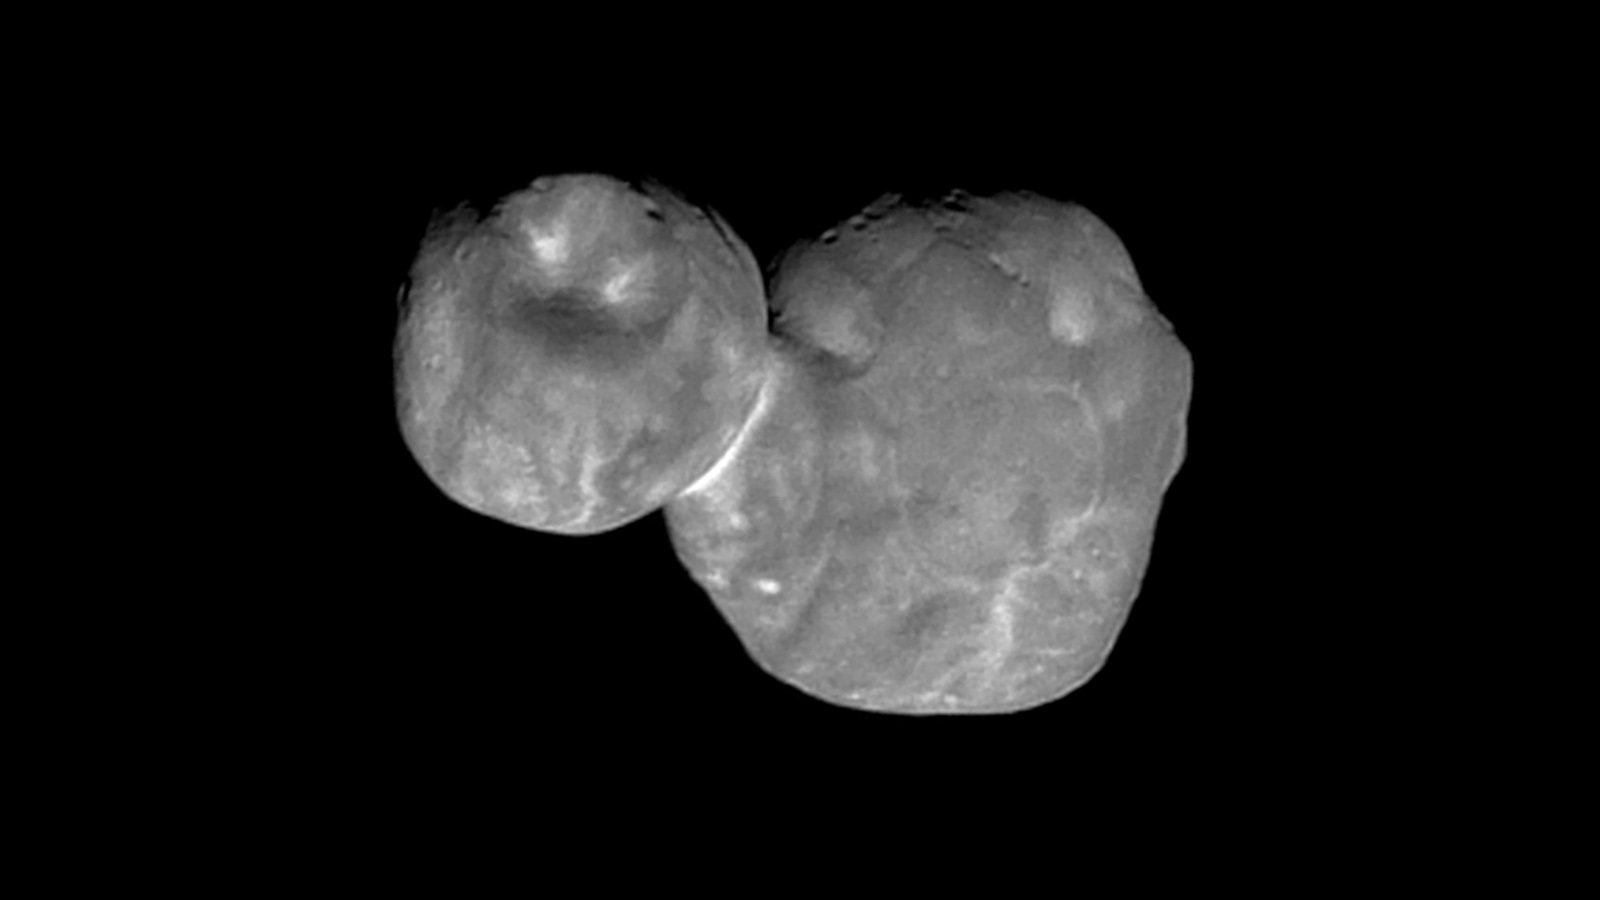
\includegraphics[width=\linewidth]{figures/819_MU69_1600.jpg}
\caption[Shot description of the figure 1.2.]{Long description of figure 1.2 (Ultima Thule captured by New Horizons). Note: there is a short description which will show on your list of figures. Note: in the  \textbackslash{includegraphics} command, use \textbackslash{linewidth} instead of \textbackslash{textwidth} to occupy almost the entire field of view. Image taken from \url{https://solarsystem.nasa.gov/system/news_items/main_images/819_MU69_1600.jpg}.}
\label{fig2}
\end{figure*}
\end{landscape}

\subsection{A Set of Subfigures}
Figure~\ref{fig3} is an example of a set of subfigures. You can cite the panels individually: Figure~\ref{fig3-a}, Figure~\ref{fig3-b}, and Figure~\ref{fig3-c}.


\begin{figure*}[htb!]
\center
\begin{subfigure}{0.67\linewidth}
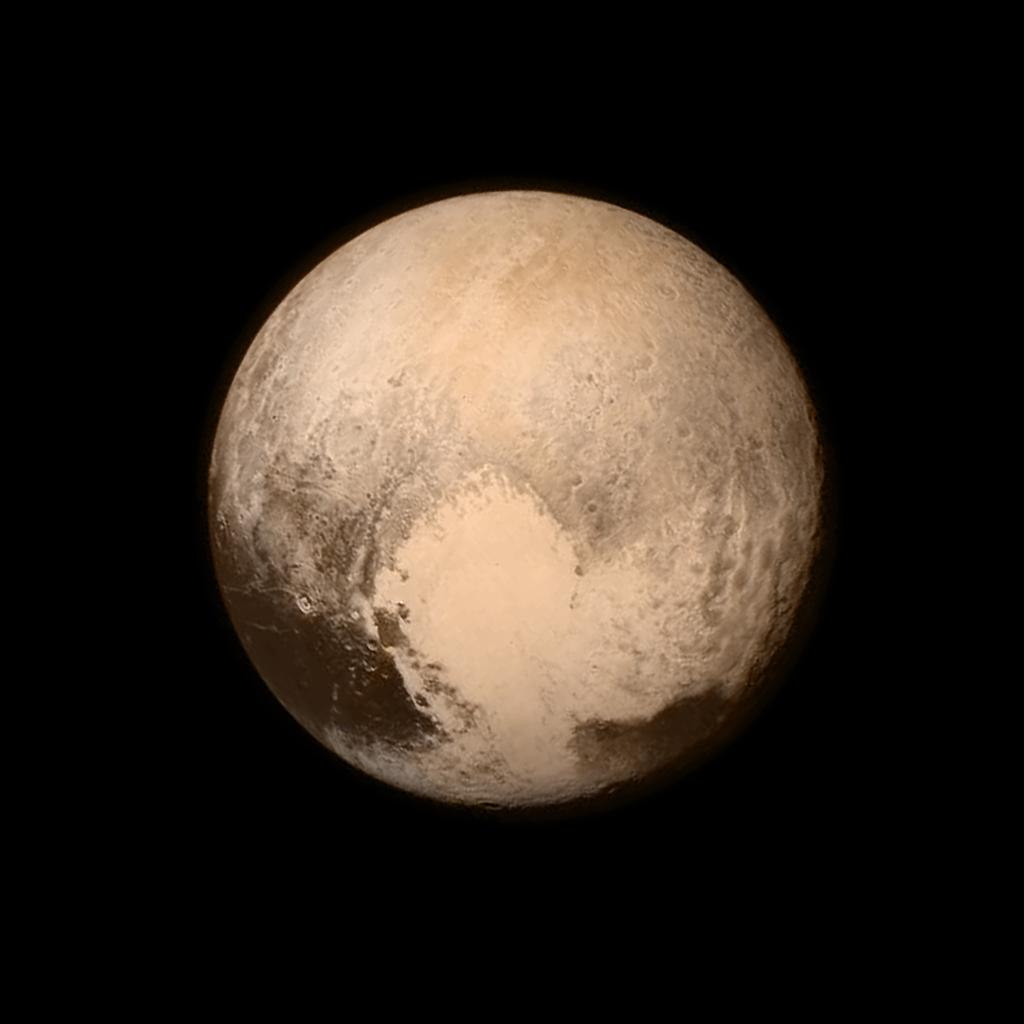
\includegraphics[width=\textwidth]{figures/PIA19708-orig.jpg}
\caption{Caption 1.}\label{fig3-a}
\end{subfigure}
\begin{subfigure}{0.35\linewidth}
\center
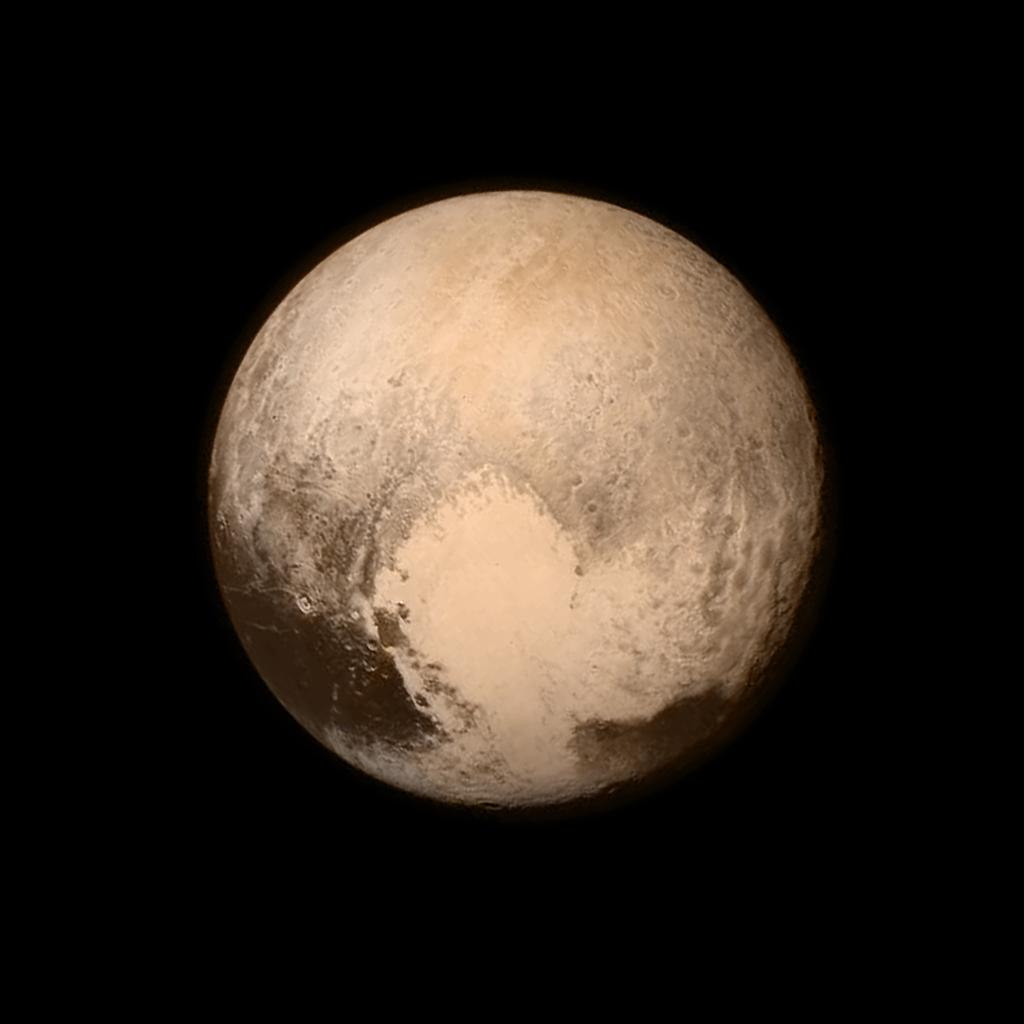
\includegraphics[width=\textwidth]{figures/PIA19708-orig.jpg}
\caption{Caption 2.}\label{fig3-b}
\end{subfigure}
\begin{subfigure}{0.24\linewidth}
\center
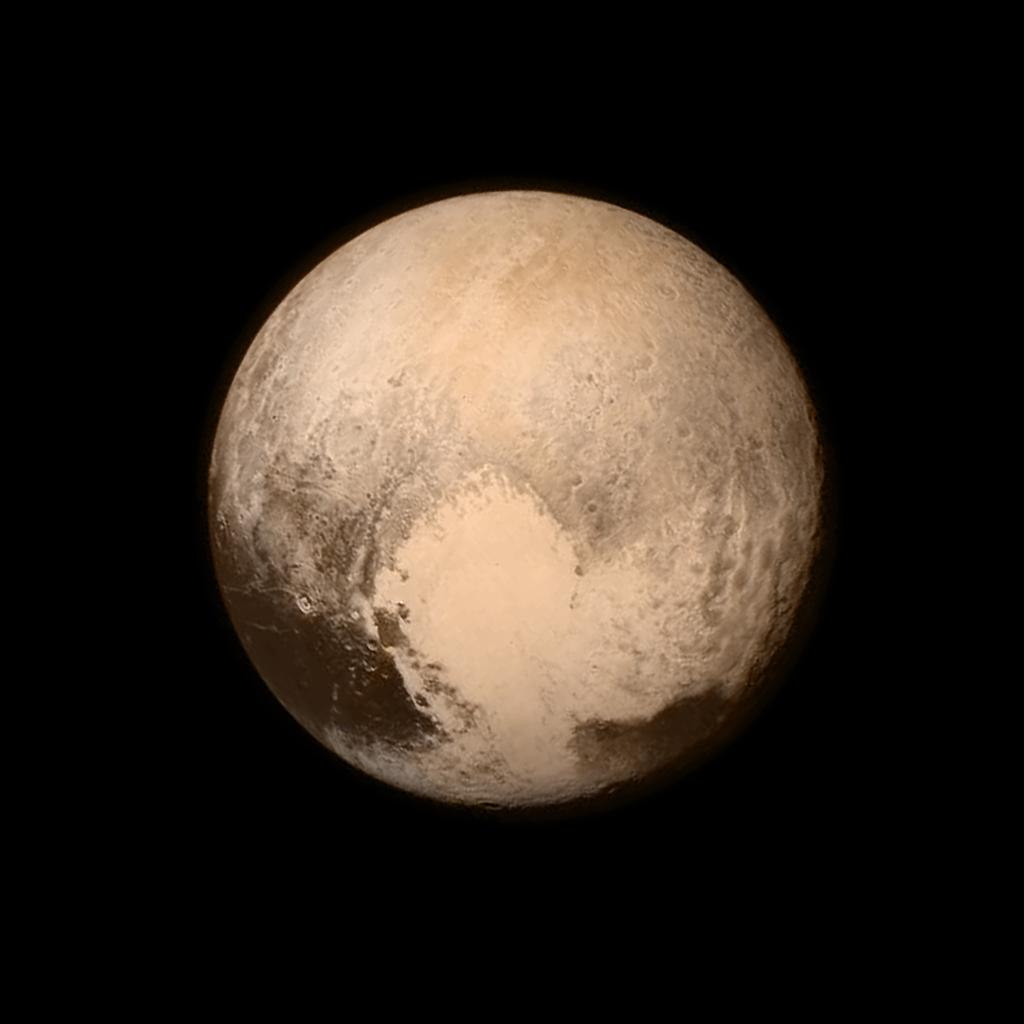
\includegraphics[width=\textwidth]{figures/PIA19708-orig.jpg}
\caption{Caption 3.}\label{fig3-c}
\end{subfigure}
\caption[Short description of figure 1.3.]{Long description of figure 1.3.}\label{fig3}
\end{figure*}
\section{Citing Chapters}
Chapter~\ref{chapter-apj} has the citations in the Astrophysical Journal\footnote{\url{https://iopscience.iop.org/journal/0004-637X}} (ApJ) style, it also shows how to use a long table. Chapter~\ref{chapter-apj-dup} has a normal table and two figures side by side.
